\documentclass[11pt,a4paper]{article}

\usepackage[polski]{babel}
\usepackage[T1]{polski}
\usepackage[utf8]{inputenc}
% \usepackage{fontspec}
\usepackage{amsmath}
\usepackage{hyperref}
\usepackage{graphicx}
\usepackage{algorithm}
\usepackage[noend]{algpseudocode}
\usepackage{tikz}
\usepackage{wrapfig}

\graphicspath{ {figures/} }
\numberwithin{equation}{section}
\numberwithin{figure}{section}
\makeatletter
\crefname
\renewcommand{\ALG@name}{Algorytm}
\hypersetup{
    colorlinks=true,
    linktoc=all,
    citecolor=black,
    filecolor=black,
    linkcolor=black,
    urlcolor=black
}
\graphicspath{ {../image} }
\setcounter{secnumdepth}{5}

\title{Optymalizacja wykorzystania materiału w procesie rozkroju rur}
\author{Jakub Pelczar}
\date{\today\\v0.3}

\begin{document}

\maketitle
\tableofcontents

\section{Wstęp}

\section{Knapsack Problem - Problem plecakowy}
Problem plecakowy jest zagadnieniem optymailzacyjnym. Problem ten swoją nazwę wziął z analogii do rzeczywistego problemu pakowania plecaka. Rozwiązując ten problem zarówno w praktyce jak i teorii trzeba zachować reguły określające ładowność plecaka dotyczące objętości i nośności plecaka. Knapsack Problem zaczął być intensywnie badany po pionierskiej pracy Dantziga\cite{DantzigArticle} w późnych latach 50 XX wieku. Znalazł on natychmiast zastosowanie w przemyśle oraz w zarządzaniu finansami. Z teoretycznego punktu widzenia, problem plecakowy często występuję jako relaksacja róznorodnych problemów programowania całkowitego\cite{PisingerThesis}.
\subsection{Zastosowanie}
Problem plecakowy stosowany jest nie tylko w sytuacji wynikającej bezpośrednio z nazwy. Znajduje on zastosowanie w wielu dziedzinach życia oraz nauki. Diffi i Helman\cite{DiffieHelmanArticle} w 1976 roku oraz Merkle i Helman\cite{MerkleHelmanArticle} w 1978 roku zaproponowali problem plecakowy jako podstawę do enkrypcji kluczy prywatnych. Jednakże podejście to w latach późniejszych zostało złamane przez środowisko kryptograficzne i jego miejsce zajęły bardziej odporne algorytmy.

"Knapsack problem" jest stosowany również podczas załadunku kontenerów służacych do przewozu materiałów drogą morską. Ładowność oraz gabaryty ładowanych elementów są ograniczane przez budowę i wytrzymałość kontenera.

Problem ten stosowany jest również w dziedzinie finansów. Jest on podstawowym narzędziem do optymalizacji portfela inwestycyjnego. Poprzez uogólnienie i modyfikacje problemu plecakowego zjawiska ekonomiczne mogą być modelowane z większą dokładnością. Przykładowo możliwe jest zakupienie 0, 1, 2 lub więcej akcji inwestycyjnych, a zakup kolejnych akcji może przynieść obniżenie przychodu.

Wiele problemów związanych z planowaniem może być przyrównana do problemu plecakowego gdzie czas wykonywania operacji na maszynie jest zasobem deficytowym. Jest on szczególnie uwydatniony gdy od aktywności maszyny zależy kapitał przedsiębiorstwa. Poprzez rozwiązanie problemu plecakowego możliwe jest przewidzenie zapotrzebowania na materiały podaczas procesu tak aby warunki zamówinia zostały spełnione\cite{BartholdiChapter}.

Kolejnym zagadnieniem wynikającym z problemu plecakowego jest problem optymalnego rozkroju, zostanie on przedstawiony w rozdziale \ref{sec:cuttingStockProblem}.
\subsection{Różnorodność problemu plecakowego}
Wszystkie elementy z rodziny tego problemu wymagają pewnego zestawu elementów które mogą zostać wybrane w taki sposób że zysk zostanie zmaksymalizowany, a pojemość placaka lub plecaków nie zostanie przekroczona. Wszystkie typy problemu należą do rodziny problemów $NP-trudnych$ co oznacza, że raczej nispotykane jest rozwiązanie problemu z użyciem algorytmów wielomianowych. Możliwe są różne warinaty problemu zależna od rozmieszczenia elementów oraz ilości plecaków\cite{PisingerThesis}:
\begin{itemize}
  \item \textit{Problem plecakowy 0-1} - każdy element może być wybrany tylko raz. Problem polega na wyborze $n$ elementów dla których suma profitów $p_j$ jest największa, bez konieczności osiągnięcia całkowitej pojemności $c$. Może być sformułowany jako problem maksymalizacji:
  \begin{equation}\label{01Knapsack}
    \begin{aligned}
      & \textrm{maksymalizacja} & & \sum_{j=1}^n p_jx_j, \\
      & \textrm{w odniesieniu do} & & \sum_{j=1}^n w_jx_j \le c, \\
      &&& x_j \in \{0,1\},& j = 1,\dots,n \\
    \end{aligned}
  \end{equation}
  gdzie $x_j$ jest wartością binarną. Jeżeli $x_j = 1$ wtedy $j$-ty element powinien znaleźć się w plecaku, w innym przypadku $x_j = 0$.
  \item \textit{Ograniczony problem plecakowy} - każdy element może być wybrany ograniczoną ilość razy. Zmianą w obecnym problemie względem problemu 0-1 jest ograniczona $m_j$ ilość elementów $j$:
  \begin{equation}\label{boundedKnapsack}
    \begin{aligned}
      & \textrm{maksymalizacja} & & \sum_{j=1}^n p_jx_j, \\
      & \textrm{w odniesieniu do} & & \sum_{j=1}^n w_jx_j \le c, \\
      &&& x_j \in \{0,1\dots,m_j\},& j = 1,\dots,n \\
    \end{aligned}
  \end{equation}
  \item \textit{Nieograniczony problem plecakowy} - jest rozszerzeniem problemu ograniczonego o nielimitowaną liczbę dostępnych elementów:
  \begin{equation}\label{unboundedKnapsack}
    \begin{aligned}
      & \textrm{maksymalizacja} & & \sum_{j=1}^n p_jx_j, \\
      & \textrm{w odniesieniu do} & & \sum_{j=1}^n w_jx_j \le c, \\
      &&& x_j \in \mathbb{N}_0,& j = 1,\dots,n \\
    \end{aligned}
  \end{equation}
  Każda zmienna $x_j$ w metodzie niograniczonej zostanie ograniczona poprzez pojemność $c$, gdy waga każdego z elementów jest równa przynajmniej jeden. W ogólnym przypadku transformacja problemu nieograniczonego w ograniczony nie przynosi korzyści
  \item \textit{Problem plecakowy wielokrotnego wyboru} - elementy powinny być wybierane z klas rozłącznych. Problem ten jest generalizacją problemu 0-1. Możliwy jest wybór dokładnie jednego elementu $j$ z każdej grupy $N_i$, $i=1,\dots,k$:
  \begin{equation}\label{multichoiceKnapsack}
    \begin{aligned}
      & \textrm{maksymalizacja} & & \sum_{i=1}^k \sum_{j \in N_i} p_{ij}x_{ij}, \\
      & \textrm{w odniesieniu do} & & \sum_{i=1}^k \sum_{j \in N_i} w_{ij}x_{ij} \le c, \\
      &&& \sum_{j \in N_i} x_{ij} = 1, & i =1,\dots,k, \\
      &&& x_j \in\{0,1\},& i = 1,\dots,k, \quad j \in N_i. \\
    \end{aligned}
  \end{equation}
  Zmienna binarna $x_{ij} = 1$ określa że $j$-ty element został wybrany z $i$-tej grupy. Ograniczenie $\sum_{j \in N_i} x_{ij} = 1, \quad i =1,\dots,k$ wymusza wybór dokładnie jednego elementu z każdej grupy.
  \item \textit{Wielokrotny problem plecakowy} - mozliwość wypełnienia wielu pleckaków. Jeśli jest możliwość załadowania $n$ elmentów do $m$ pleckaów o róznych pojemnościahc $c_i$ w taki sposób że zysk będzie jak największy:
  \begin{equation}\label{multiKnapsack}
    \begin{aligned}
      & \textrm{maksymalizacja} & & \sum_{i=1}^k \sum_{j \in N_i} p_{ij}x_{ij}, \\
      & \textrm{w odniesieniu do} & & \sum_{j=1}^n  w_jx_{ij} \le c_i, & i =1,\dots,m \\
      &&& \sum_{j \in N_i} x_{ij} \le 1, & i =1,\dots,k, \\
      &&& x_j \in\{0,1\},& i = 1,\dots,m, \quad j =1,\dots,n. \\
    \end{aligned}
  \end{equation}
  Zmienna $x_{ij} = 1$ określa że $j$-ty element powinien zostać umiesczony w $i$-tym plecaku, podczas gdy ogranicznie $\sum_{j=1}^n  w_{ij}x_{ij} \le c_i$ zapewnia że restrykcja dotycząca pojemności plecaka zostanie zachowana. Ogranicznie $\sum_{j \in N_i} x_{ij} \le 1$ zapewnia że każdy element zostanie wybrany tylko raz.
  \item \textit{Bin-packing problem} - bardzo często spotykana wersja problemu plecakowego/ Problem ten polega na umieszczeniu $n$ elementów w jak najmniejszej liczbie opakowań:
  \begin{equation}\label{binPacking}
    \begin{aligned}
      & \textrm{maksymalizacja} & & \sum_{i=1}^n y_i \\
      & \textrm{w odniesieniu do} & & \sum_{j=1}^n w_jx_{ij} \le cy_i, & i=1,\dots,n, \\
      &&& \sum_{i=1}^n x_{ij} = 1, & j=1,\dots,n, \\
      &&& y_i \in \{0,1\}, & i=1,\dots,n, \\
      &&& x_{ij} \in \{0,1\} & i=1,\dots,m, \quad j = 1,\dots,n,
    \end{aligned}
  \end{equation}
  gdzie $y_i$ określa czy $i$-te opakowanie zostało użyte, a $x_{ij}$ stanowi czy $j$-ty element powinen zostać umieszcozny w $i$-tym opakowaniu
  \item \textit{Welokrotnie ograniczony problem plecakowy} - najbardziej ogólny typ który jest problemem programowania całkowitego z dodatnimi współczynnikami:
  \begin{equation}\label{generalKnapsack}
    \begin{aligned}
      & \textrm{maksymalizacja} & & \sum_{j=1}^n p_jx_j, \\
      & \textrm{w odniesieniu do} & & \sum_{j=1}^n w_jx_j \le c_i, & i=1,\dots,m, \\
      &&& x_j \in \mathbb{N}_0, & j = 1,\dots,n. \\
    \end{aligned}
  \end{equation}
\end{itemize}

\subsection{Możliwe rozwiązania}

Problem plecakowy należy do grupy problemów $\mathcal{NP}$-Trudnych. Rozwiązanie problemów z tej grupy jest co najmniej tak trudne, jak rozwiązanie każdego problemu z całej klasy $\mathcal{NP}$. Problem $\mathcal{NP}$-Trudny to problem obliczeniowy dla którego znalezienie rozwiązania problemu nie jest możliwe z wielomianową złożonościa obliczeniową. Problemy $\mathcal{NP}$-Trudne obejmują zarówno problemy decyzyjne jak również problemy przeszukiwania czy też problemy optymalizacyjne.

Rozwiązanie problemu plecakowego jest możliwe przy użyciu różnych metod:
\begin{itemize}
  \item \textit{Metoda podziału i ograniczeń} - Metoda ta często jest stosowana do problemu plecakowego od momentu gdy Kolesar \cite{KolesarArticle} zaprezentował pierwszy algorytm w 1967 roku.
  \item \textit{Programownaie dynamiczne} - Gdy zostaną dodane warunki brzegowe wtedy algorytm ten staje się "zaawansowaną" formą metody podziału i ograniczeń.
  \item \textit{Relaksacja przestrzeni stanów} - relaksacja programowani dynamicznego gdzie współczynniki są skalowane przez pewną stałą wartość.
\end{itemize}

\subsubsection{Metoda podziału i ograniczeń}
Algorytm ten polega na wypisaniu wszystkich możliwych rozwiązań używając struktury drzewiastej. Algorytm przechodzi kolejno po gałęziach drzewa które reprezentują podzbiory rozwiązania. Każda gałąź jest sprawdzana zadanymi warunkami brzegowymi i jest odrzucana jeśli nie poprawi rozwiąznaia. Przedstawione zostanie rozwiązanie ogólnego problemu plecakowego (\ref{generalKnapsack}) \cite{ChvatalBook}. 

\subsubsection{Programowanie dynamiczne}
Metoda ta używana jest w przypadku gdy problem można podzielić na małe podproblemy które można rozwiązać rekursywnie. Rozwiązanie optymalne podproblemu jest również optymalnym rozwiązaniem problemu głównego. Przedstawione zostanie rozwiązanie problemu plecakowego rodzaju 0-1 \cite{GoddardLecture}.

Jeśli elementy są oznaczone jako $1,\dots,n$ wtedy podproblem będzie odpowiedzialny za znalezienie optymalnego rozwiązania dla $S_k = \{1,2,\dots,k \}$. Niemożliwe jest opisanie rozwiązania końcowego $S_n$ na podstawie podproblemów $S_k$. Rekursywne sformułowanie podproblemu:
\begin{equation}\label{recursiveDynamic}
  \begin{aligned}
    B[k,w] =
    \begin{cases}
    & B[k-1,w] \quad \textrm{jeśli} \quad w_k > w, \\
    & max\{B[k-1,w], B[k-1,w-w_k] + b_k\} \quad \textrm{jeśli} \quad  w_k \le w.
    \end{cases}
  \end{aligned}
\end{equation}
Z powyższego równania wynika że najlepszy podzbiór podproblemu $S_k$ z całkowitą wagą $w$ jest najlepszym podzbiorem dla $S_{k-1}$ którego całkowita waga wymosi $w$ lub jest najlepszym podzbiorem dla $S_{k-1}$ którego całkowita waga wynosi $w-w_k$ plus $k$-ty element. Złożoność programowania dynamicznego to $O(n*W)$. Algorytm jako dane wejściowe przyjmuje maksymalną wartość ciężaru $W$, oraz dwie listy: listę wag $w_1,\dots,w_n$ oraz odpowiadającą jej listę zysku $b_1,\dots,b_n$.
\begin{algorithm}
  \caption{Programowanie dynamiczne - problem plecakowy 0-1}
  \begin{algorithmic}[1]
    \For {w := 0 TO W}
      \State B[0,w] := 0
    \EndFor
    \For {i := 1 TO n}
      \State B[i,0] := 0
    \EndFor
    \For {i := 1 TO n}
      \For {w := 0 TO W}
        \If {$w_i \le w$}
          \If {$b_i + B[i-1,w-w_i] > B[i-1,w]$}
            \State $B[i,w] := b_i + B[i-1,w-w_i]$
          \Else
            \State $B[i,w] := B[i-1,w]$
          \EndIf
        \Else
          \State $B[i,w] := B[i-1,w]$
        \EndIf
      \EndFor
    \EndFor
  \end{algorithmic}
\end{algorithm}

\section{Cutting Stock Problem - Problem optymalnego rozkroju}
\label{sec:cuttingStockProblem}

% \section{Metoda "Brutal Force"}
\subsection{Algorytm wyjściowy}
Metoda ta opiera się zarówno na intuicji jak i na rozwiązaniu zaproponowanym przez Dantziga dla problemu plecakowego \cite{DantzigArticle}. Jest to metoda która w prosty sposób - nie używając złożonych modeli matematycznych, pozwala osiągnąć optymalny rozkrój materiału.

Pierwszym krokiem jest posortowanie malejąco po długości elementów wyściowych. $l_1 \ge l_2 \ge ... \ge l_m$

Drugim krokiem jest pobranie pierwszego elementu z kolejki i sprawdzenie, jak wiele razy dana długość zawiera się w długości elementu bazowego. Obliczone zostaje ile materiału pozostało w elemencie bazowym. Pobierany jest następny odcinek z kolejki. Zostaje sprawdzone ile razy zawiera się w pozostałej długości.
\begin{equation}\label{base_dantizg}
a_1 = [L/l_1], a_2 = [(L-l_1*a_1)/l_2], a_3 = [(L-(l_1*a_1+l_2*a_2))/l_3], ...
\end{equation}
Kroki te powtarzane są dopóki kolejka się nie skończy.

Każdy element wyjściowy posiada określoną liczebność jaką powinien osiągnąć na końcu procesu. Jeśli licznik jest równy zeru wówczas długość jest pomijana. Koniecznie jest sprawdzenie czy otrzymany wynik jest mniejszy lub równy od wymaganej ilości:
\begin{itemize}
  \item Jeśli stwierdzenie jest prawdziwe - długość z której elementy są wycinane zostanie zmniejszona o liczbę wystąpień wykrojów w aktywności (zestawie elementów wykroju) pomnożoną przez długość elementu, a licznik wymaganych odcinków danej długości zostanie zmniejszony o odpowiednią liczbę wystąpień
  \item Jeśli stwierdzenie jest fałszywe - długość z której elementy są wycinane zostanie zmniejszona o liczbę dostępnych wykrojów pomnożoną przez długość elementu, a licznik wymaganych odcinków danej długości zostanie ustawiony na zero.
\end{itemize}
Po zakończeniu przebiegu algorytmu dla danego układu wykrojów określa się ile razy dana aktywność może zostać użyta. Można to wyznaczyć poprzez obliczenie $g = min\{z_i/a_i\}, i \in {0,..,m}$, gdzie $z$ to pozostała ilość wykrojów elementu $i$, $a$ to ilość wykrojów elementu $i$ w danej aktywności. Następnie zmniejsza się o $g$ licznik dostępnych odcinków danego elementu dla którego $a_i > 0$.

Cały proces powtarzany jest do momentu aż wszytskie wymagane elementy zostaną wycięte.

\subsection{Rozszerzenie o szerokość cięcia}
W warunkach rzeczywistych elementy wycinane są za pomocą ostrza które ma niezerową szerokość. Wówczas metodę obliczania należy rozszerzyć jeśli ma odpowiadać warunkom rzeczywistym. Szerokość cięcia wlicza się w odpad. Jest kilka przypadków wliczania szerokości ostrza.

Jeżeli element jest równy długości bazowej wówczas nie wlicza się szerokości cięcia. Natomiast jeżeli materiał bazowy ma zostać pocięty na kilka elmentów wówczas do każdego dolicza się szerokość cięcia. Szczególnym przypadkiem jest, gdy ostatni element wraz z szerokością ostrza jest dłuższy niż długość odcinka, który został po wycięciu wcześniejszych elementów.

Gdyby szerokość cięcia nie zostałą uwzględniona w obliczeniach wówczas dla elementu wejściowego o długości 6000mm i wymaganych odcinkach 4500mm oraz 1500mm, obie długości zostały wycięte z jednego segmentu materiału bazowego. Skutkiem takiego postępowania byłby element krótszy o szerokość ostrza. Zazwyczaj dłuŋość ta może być akceptowana jako toleracncja dokładności maszyny. Jednak dla poprawności obliczeń wielkość ta powinna zostać uwzględniona.

\subsection{Rozszerzenie o wiele długości bazowych}
Dla zmniejszenia odpadu można użyć kilku długości bazowych. Rozszerzenie to wprowadza następująca zmianę algorytmu: obliczenia układu muszą zostać powtórzone dla każdego elementu wejściowego. Następnie wybierany jest ten rozkrój, który daje mniejszy odpad. Modyfikacja ta znacząco wpływa na wydajność metody. Jeżeli $n$ oznacza złożoność obliczeniową podstawowego algorytmu, a $m$ oznacza liczbę odcinków wejściowych, wówczas nowa złożonośc obliczeniowa wynosi $m*n$.

\subsection{Rozszerzenie o cenę materiału wsadowego}
Rozszerzenie to wprowadza zmianę koncepcyjną. Każdy element bazowy posiada cenę za metr bieżący materiału, umożliwia to obliczenie kosztu odpadu i wybranie tańszej opcji wykroju.

\subsection{Przykład}

% \newcommand{\mf}[1]{\textbf{\textit{#1}}}
\newcommand{\tsub}[1]{\textsubscript{#1}}
\newcommand{\tsuper}[1]{\textsuperscript{#1}}

\section{Metoda "Delayed Column Generation"}

\subsection{Algorytm}

\begin{equation}\label{length_eq}
L \ge l_1a_1+\dots+l_ma_m
\end{equation}

\begin{equation}\label{cost_eq}
b_1a_1+\dots+b_ma_m > c
\end{equation}

\begin{enumerate}
\item Określnie $m$ poczatkowych rokrojów i ich kosztu w następujący sposób: dla każdego $i$ wybranie długości bazowej $L_j$ dla której $L_j > l_i$ i określenie $i$-tego rokroju jako wycięcie $a_{ii} = [L_j / l_i]$ elementów o długości $l_i$ z długości $L_j$. Koszt $i$-tego rozkroju będzie równy kosztowi $c_j$ długości $L_j$ z której $i$-ta operacja wycina odcinki o długości $l_i$.
\item Uformowanie macierzy \mf{B}
\[
\begin{matrix}
1 & -c_1  & -c_2  & \dots & -c_m \\
0 & a_{11}  & 0 & \dots & 0 \\
0 & 0 & a_{22}  & \dots & 0 \\
\vdots&\vdots&\vdots&\ddots&\vdots \\
0 & 0 & 0 & \dots & a_{mm}
\end{matrix}
\]
gdzie $a_{ii}$ jest ilością odcinków o długości $l_i$ wyciętych w $i$-tym rozkroju z długości bazowej o koszcie $c_j$. Ostatnie $m$ kolumn jets powiązane z rozkrojami. Dane te będą aktualizowane gdy zostanie znaleziony wynik który poprawi rozwiązanie.

Utworzenie $m$ $m+1$ wymiarowych wektorów kolumnowych \mf{S\tsub{1}},...,\mf{S\tsub{m}} odnoszących się do zmiennych dodatkowych, gdzie \mf{S\tsub{i}} posiada same zera z wyjątkiem wiersza $(i+1)$ w którym jest $-1$. Dodatkowo utworzenie $m+1$ wymiarowego wektora kolumnowego \mf{N'} który jako pierwszy element przyjmuje 0, a w następnych $i$-tych wierszach posiada wartośic $N_i$.

Obliczenie \mf{B}\tsuper{-1} która wynosi:
\[
\begin{matrix}
1 & c_1/a_{11}  & c_2/a_{22}  & \dots & c_m/a_{mm} \\
0 & 1/a_{11}  & 0 & \dots & 0 \\
0 & 0 & 1/a_{22}  & \dots & 0 \\
\vdots&\vdots&\vdots&\ddots&\vdots \\
0 & 0 & 0 & \dots & 1/a_{mm}
\end{matrix}
\]

Niech $\mf{N} = \mf{B}^{-1} \cdotp \mf{N'}$. Sprawdzając czy pierwszy element z $\mf{B}\tsuper{-1} \cdotp \mf{P}$ jest dodatni można określić czy istnieje możliwość polepszenia rozwiązania. Wektor kolumnowy \mf{P} jets wektorem złożonym ze zmiennych nieuzytych w bieżącym rozwiązaniu, np. pierwszy element to negatywny koszt, a pozostałe $m$ wierszy jest równe zmiennym $a_{ij}$.

\item Z powyższego puntku wynika że jeśli $i$-ta zmienna dodatkowa która nie wchodzi w skład rozwiązania może ulepszyć rozwiązanie wtedy i tylko wtedy gdy $(i+1)$ element pierwszego wiersza \mf{B}\tsuper{-1} jest ujemny.

\item Jeśli nie jest możliwe polepszenie rozwiązania nalezy określić czy wprowadznie nowego rozkroju ulepszy bieżące rozwiązanie. Jets to możliwe poprzez sprawdznie czy dla $L$ z kosztem $c$ istnieje rozwiązanie nierówności \ref{length_eq} oraz \ref{cost_eq}, gdzie $b_1,\dots,b_m$ to ostatnie $m$ elementów w piwerwszym wierszu \mf{B}\tsuper{-1}. Jeśli te nierównoście nie posiadają rozwiąania dla dowolnej długości $L_1,\dots,L_k$ z kosztem odpowiednio $c_1,\dots,c_m$ wtedy bieżące rozwiązanie jest minimum. Rozwiązanie i jego koszt jest określone poprzez \mf{N}, gdzie pierwszy wiersz to koszt, a pozostałe $m$ wierszy jest, w kolejności, odpowiednimi wartościami $m$-tej kolumny z \mf{B}\tsuper{-1}.

Jeśli nowy rozkrój poprawi rozwiązanie wtedy formowany jest nowy wektor \mf{P} ze współczynnikami, w kolejności $-c,a_1,a_2,\dots,a_m$.

\item Wprowadznie zarówno dodatkowej zmiennej jak i nowego rozkroju może poprawić rozwiązanie. W obu przypadkach \mf{P} będzie kolumnowym wektorem ze zmiennymi. Dla określenia nowych \mf{B}\tsuper{-1} oraz \mf{N} które opisują ulepszone rozwiązanie i jego koszt, co pozawala na przejście przez kkroki 3, 4 oraz kontynujacje kroku 5 w nastepujący sposób: Obliczenie $\mf{B}\tsuper{-1} \cdotp \mf{P}$ - niech elementy wynikime będą elementy $y_1,\dots,y_m,y_{m+1}$ oraz niech elementami bierzącego wektora \mf{N} będą $x_1,\dots,x_m,x_{m+1}$. Ustalenie $i$, $ i \ge 2$ dla każdego $y_i > 0$, $x_i \ge 0$ oraz $x_i/y_i$ jest najminiejsze i przypisanie tej wartości do zmiennej $k$. Minimalny stosunek powinien być zerem aby można było wykorzystać metodę degeneracji.

Jeśli stosunek nie jest równy zero wtedy $k$-ty element wektora \mf{P}, $y_k$ będzie elementem wokół którego zajdzie eliminacja Gaussa odbywająca się równocześnie na \mf{B}\tsuper{-1}, $\mf{B}\tsuper{-1} \cdotp \mf{P}$ oraz \mf{N}. Eliminacja ta przebiega na macierzy $(m+1) \times (m+3)$ wymiarowej \mf{G} uformowanej z \mf{B}\tsuper{-1} poprzez dołączenie kolumn $\mf{B}\tsuper{-1} \cdotp \mf{P}$ oraz \mf{N}. Pierwsze $m+1$ kolumn \mf{G'} formuje nową macierz \mf{B}\tsuper{-1}, a kolumna $m+2$ to nowy wektor \mf{N}. Zależność między kolumnami \mf{B}\tsuper{-1} a rozkrojami lub zmiennymi dodatkowymi jets aktualizowana poprzez usunięcie $k$-tej kolumny i podmienieniu jej na nowy rozkruj lub zmienną dodatkową.

Degeneracja w razie wystąpienia może zostać obsłużona w tradycyjny sposób. Pewne środki ostrożności powinny zostać podjęte w celu uniknięcia cykliczności. Nowa kolumna \mf{N}\tsuper{1} z dodatnimi elementami $x_1',\dots,x_{m+1}'$ która jest niezależna od \mf{N} jest dołączana do \mf{G}, następnie dokonywany jest wybór takiego $y_i > 0$ dla którego $x_i = 0$ jest elementem osiowym jets dokonywany na podstawie takiego $i$ dla którego $x_i' > 0$ oraz $x_i'/y_i$ jest najmniejsze. Gdy element osiowy zostanie wybrany, wówczas eliminacja Gaussa zachodzi tak jak w poprzednim przypadku na powiększonej macierzy \mf{G}. Dodatkowa kolumna jest przechowywane w \mf{G} dopóki istnieje takie $i$ dla którego $x_i/y_i$ jest dodatnie i skończone, jeśłi warunek ten jest spełniony wówczas kolumna zostaje usunięta. Powinno to nastąpić w przypadku gdy nie istnieje takie $i$ dla którego $x_i/y_i$ oraz $x_i'/y_i$ są dodatnie i skończone. Wówczas powinna zostać dodana kolumna \mf{N}\tsuper{2} nizależna od \mf{N} oraz \mf{N}\tsuper{1}. Podobnie dowolna liczba kolumn może zostac dodana i usunięta gdy przestanie byc potrzebna. Dopóki kolumny są niezależne w czasie dodawania i pozostają takie po eliminacji Gaussa, nie potrzeba więcej jak $m$ nowych kolumn. Każda dodana kolumna definiuje nowy problem liniowy który eliminuje problem cykliczności tak długo aż degeneracja nie wystąpi.

\end{enumerate}

\subsection{Metody użyte w implementacji}

\paragraph{Dwufazowa metoda simplex}
\paragraph{Metoda podziału i ograniczeń}

\subsection{Przykład}

\section{Wyniki}

Niniejsza sekcja przedstawia i porównuje wyniki otrzymane z eksperymentu. Metody wchodzące w skład porównania to "Delayed Column Generation" (\hyperref[sec:dcg]{rozdział~\ref*{sec:dcg}}). oraz "Brutal Force" (\hyperref[brutalForce]{rozdział~\ref*{brutalForce}}). Warunki przeprowadzenia testu:
\begin{itemize}
  \item Losowo generowane odcinki wynyikowe o długości od 1 do 21 cm, przy liczebności od 1 do 200 elementów.
  \item Losowo generowane 5 długości początkowych od 22 do 42 cm, o koszcie od 1\$. Każda długość posiada inną cenę.
  \item Obie metody testowane są takimi samymi danymi.
  \item Wykonano 27 różnych rozkrojów.
  \item Czas wykonania mierzony od dostarczenia danych do zwrócenia wyniku, bez uwzględnianienia czasu przygotowania danych oraz ich zapisu.
  \item Warunki sprzętowe:
  \begin{itemize}
    \item Procesor: Intel Core i5-6500u @ 2.30 GHz x 2 z technologią HT.
    \item RAM: 16 GB (15.2 GB).
    \item System operacyjny: Linux Mint 18.1 Cinammon 64-bit.
  \end{itemize}
  \item Język implementacji: Kotiln 1.0.5 (JVM), Java 8 (Oracle Java 1.8\_121).
  \item Aplikacja jednowątkowa.
\end{itemize}
\subsection{Porównanie}

Dane z tabeli \ref{tab:result} przedstawiają porównanie podstawowych statystyk dla każdego kroku eksperymentu. Natomiast tabela \ref{tab:average} przedstawia średnie wartości statystyk przedstawionych w poprzedniej tabeli.

\begin{table}[]
\centering
\caption{Wyniki}
\label{tab:result}
\begin{tabular}{@{}|c|c|c|c|c|c|@{}}
\toprule
\multicolumn{2}{|c|}{\textbf{Czas (ms)}} & \multicolumn{2}{c|}{\textbf{Koszt}} & \multicolumn{2}{c|}{\textbf{Odpad}} \\ \midrule
\textit{DCG}        & \textit{BF}        & \textit{DCG}      & \textit{BF}     & \textit{DCG}      & \textit{BF}     \\ \midrule
136396              & 11                 & 1830              & 2835            & 0                 & 0               \\ \midrule
27688               & 2                  & 1719              & 2342            & 304               & 13              \\ \midrule
190893              & 3                  & 3279              & 3421            & 109               & 33              \\ \midrule
113044              & 2                  & 1936              & 5397            & 69                & 20              \\ \midrule
14453               & 5                  & 1821              & 2342            & 819               & 8               \\ \midrule
446814              & 1                  & 2912              & 4254            & 3947              & 3               \\ \midrule
20758               & 3                  & 4544              & 5050            & 1729              & 3               \\ \midrule
101468              & 2                  & 3024              & 6658            & 54                & 1               \\ \midrule
272598              & 1                  & 2324              & 2560            & 44                & 0               \\ \midrule
18424               & 1                  & 2365              & 4001            & 877               & 64              \\ \midrule
284007              & 1                  & 1802              & 4000            & 46                & 40              \\ \midrule
36820               & 6                  & 3078              & 3255            & 393               & 115             \\ \midrule
25840               & 8                  & 4068              & 6981            & 325               & 14              \\ \midrule
42254               & 16                 & 948               & 1034            & 1480              & 102             \\ \midrule
4664                & 1                  & 3174              & 3707            & 1434              & 1297            \\ \midrule
11725               & 3                  & 1377              & 2904            & 46                & 2               \\ \midrule
34074               & 6                  & 1161              & 1490            & 411               & 45              \\ \midrule
323568              & 7                  & 3072              & 3638            & 81                & 1               \\ \midrule
124059              & 4                  & 8128              & 8971            & 0                 & 51              \\ \midrule
27697               & 1                  & 830               & 3965            & 0                 & 9               \\ \midrule
169184              & 2                  & 2754              & 3255            & 0                 & 18              \\ \midrule
227189              & 7                  & 3184              & 5741            & 150               & 94              \\ \midrule
25436               & 5                  & 1235              & 1850            & 35                & 21              \\ \midrule
232145              & 3                  & 4485              & 4598            & 0                 & 4               \\ \midrule
47524               & 2                  & 2993              & 4046            & 1278              & 159             \\ \midrule
77913               & 2                  & 5002              & 5196            & 23                & 10              \\ \midrule
201725              & 1                  & 2366              & 3162            & 0                 & 14              \\ \midrule
18760               & 2                  & 5330              & 5398            & 64                & 12              \\ \bottomrule
\end{tabular}
\end{table}

\begin{table}[]
\centering
\caption{Średnie}
\label{tab:average}
\begin{tabular}{|l|c|c|}
\hline
                                           & \textbf{DCG}   & \textbf{BF}   \\ \hline
\textbf{Średni czas}                       & 116325.71      & 3.86          \\ \hline
\textbf{(DCG/BF) * 100\%}  & \multicolumn{2}{c|}{3015851.85\%} \\ \hline
\textbf{Średni koszt}                      & 2883.61        & 4001.82       \\ \hline
\textbf{(BF/DCG) * 100\%} & \multicolumn{2}{c|}{138.78\%}  \\ \hline
\textbf{Średni odpad}                      & 489.93         & 76.89         \\ \hline
\textbf{(DCG/BF) * 100\%} & \multicolumn{2}{c|}{637.16\%}    \\ \hline
\end{tabular}
\end{table}

Dane przedstawione w powyższych tabelach wskzaują jednoznacznie że, metoda brutalnej siły (dalej BF) jest szybsza niż druga metoda użyta w porównaniu. Tabela \ref{tab:average} wskazuje iż metoda opóźnieonej generacji kolumn (dalej DCG) jest średni prawie 30156 razy wolniejsza niż metoda BF. Ma to związek z nakładem obliczeniowym metody DCG. Metoda ta wykonuje wiele obliczeń macierzowych, dla każdej itereacji zachodzi odwracanie macierzy, mnożenie wektorów, eliminacja Gaussa oraz rozwiązywanie układu nierówności dwufazowa metoda sympleks. Najwyższy czas wykonania metody DCG wynodi 446814 ms, czyli ponad 7 minut. Najmniejszy czas wykonania tej samej metody przy innych danych wejściowych i zachowaniu warunków testu wynosi 4664 ms, czyli 4,7 s. Rozbieżność czasów wykonania metody DCG wskazują na silną zależność między danymi wejściowymi, a czsem wykonania. Czas wykonania metody BF jest bardzo niski, na poziomie kilkunastu milisekund, jest to związane ze spsobem wykonania. Głóœnym elementem implmentacji tej metody jest przeszukiwaniem, przechodzenie oraz uzupełnianie tablic. Operacje te są znacznie szybsze niż operacje macierzowe. Mediana czasów obu metod pokazuje że, metoda DCG nadal jest dużo wolniejsza niż BF, jednak w innej skali niż porównanie średnich. Mediana dla metody DCG to 62718.5 ms, a dla BF to 2.5 s. Metoda DCG jest ponad 25087 razy wolniejsza niż metoda BF.

Kolejna część powyższych tabel odnosi się do średniego kosztu wykroju całkowitego. Koszt uzyskany metodą BF jest średnio 1.4 razy większy niż metodą DCG. Liczba ile razy koszt jednej metody zawiera się w drugej wydaje się mały. Jednak po sprawdzeniu wielkości kosztów wynika iż, różnica między ceną rozwiązania metodą DCG oraz metodą BF wynosi 1118, 21\$. Rząd wielkości oznacza że, różnica w cenie jest znacząca. Metoda DCG jako główny cel ma minimalizację kosztu, natomiast metoda BF jak najmniejszą cenę odpadu w ujęciu bierzącecgo schematu rozkroju.

Ostatnie częsci powyższych tabel ukazują odpad powstały z rozkroju otrzymanymi schmatami. Odpad wyprodukowany z metody dCg jest ponad 6 razy większy niż odpad z metdoy BF. W jednym przypadku na 28, odpad z metdy DCG był mniejszy niż z metody BF. Tak jak zostało wspomnianie w powyższym akapicie metoda BF skupia się na minimalizacji kosztu odpadu, więc w ogólnym przypadku minimalizuje odpad.   

\begin{longtable}{lllllllll}
Base Lengths             &              &           &                  &    &    &    &   &    \\
Length                   & Cost         &           &                  &    &    &    &   &    \\
25                       & 7            &           &                  &    &    &    &   &    \\
31                       & 21           &           &                  &    &    &    &   &    \\
33                       & 9            &           &                  &    &    &    &   &    \\
36                       & 15           &           &                  &    &    &    &   &    \\
Request     &              &           &                  &    &    &    &   &    \\
Length                   & Quantity     &           &                  &    &    &    &   &    \\
2                        & 66           &           &                  &    &    &    &   &    \\
4                        & 167          &           &                  &    &    &    &   &    \\
5                        & 174          &           &                  &    &    &    &   &    \\
7                        & 151          &           &                  &    &    &    &   &    \\
9                        & 200          &           &                  &    &    &    &   &    \\
10                       & 135          &           &                  &    &    &    &   &    \\
12                       & 150          &           &                  &    &    &    &   &    \\
15                       & 26           &           &                  &    &    &    &   &    \\
17                       & 8            &           &                  &    &    &    &   &    \\
                         &              &           &                  &    &    &    &   &    \\
OUTPUT                   &              &           &                  &    &    &    &   &    \\
Used base         &              &           &                  &    &    &    &   &    \\
Length                   & Quantity     &           &                  &    &    &    &   &    \\
25                       & 305          &           &                  &    &    &    &   &    \\
33                       & 21           &           &                  &    &    &    &   &    \\
                         &              &           &                  &    &    &    &   &    \\
Output table             &              &           &                  &    &    &    &   &    \\
Quantity                 & Waste        & Used base & \multicolumn{6}{c}{Elements}    \\
14                       & 0            & 25        & 2                & 2  & 2  & 2  & 5 & 12 \\
76                       & 0            & 25        & 4                & 4  & 5  & 12 &   &    \\
4                        & 0            & 25        & 5                & 5  & 5  & 5  & 5 &    \\
16                       & 0            & 25        & 4                & 7  & 7  & 7  &   &    \\
96                       & 0            & 25        & 7                & 9  & 9  &    &   &    \\
68                       & 0            & 25        & 5                & 10 & 10 &    &   &    \\
31                       & 1            & 25        & 12               & 12 &    &    &   &    \\
13                       & 1            & 33        & 2                & 15 & 15 &    &   &    \\
8                        & 0            & 33        & 7                & 9  & 17 &    &   &    \\
                         &              &           &                  &    &    &    &   &    \\
Statistic                &              &           &                  &    &    &    &   &    \\
Exec time (ms)           & 272598       &           &                  &    &    &    &   &    \\
Total cost               & 2324         &           &                  &    &    &    &   &    \\
Waste                    & 44           &           &                  &    &    &    &   &    \\
Waste percent            & 5.289733E-05 &           &                  &    &    &    &   &    \\
                         &              &           &                  &    &    &    &   &    \\
Output elements          &              &           &                  &    &    &    &   &    \\
Length                   & Quantity     &           &                  &    &    &    &   &    \\
2                        & 69           &           &                  &    &    &    &   &    \\
4                        & 168          &           &                  &    &    &    &   &    \\
5                        & 178          &           &                  &    &    &    &   &    \\
7                        & 152          &           &                  &    &    &    &   &    \\
9                        & 200          &           &                  &    &    &    &   &    \\
10                       & 136          &           &                  &    &    &    &   &    \\
12                       & 152          &           &                  &    &    &    &   &    \\
15                       & 26           &           &                  &    &    &    &   &    \\
17                       & 8            &           &                  &    &    &    &   &    \\
                         &              &           &                  &    &    &    &   &    \\
Cost decreasing &              &           &                  &    &    &    &   &    \\
Step                     & Cost         &           &                  &    &    &    &   &    \\
0                        & 2755.0166    &           &                  &    &    &    &   &    \\
1                        & 2692.1833    &           &                  &    &    &    &   &    \\
2                        & 2661.5166    &           &                  &    &    &    &   &    \\
3                        & 2437.5166    &           &                  &    &    &    &   &    \\
4                        & 2343.0166    &           &                  &    &    &    &   &    \\
5                        & 2324.7388    &           &                  &    &    &    &   &    \\
6                        & 2317.6765    &           &                  &    &    &    &   &    \\
7                        & 2314.585     &           &                  &    &    &    &   &    \\
8                        & 2303.9917    &           &                  &    &    &    &   &
\end{longtable}


\subsection{Wnioski}

\section{Opis implementacji}
\label{sec:implemenation}
Aplikacja została napisana przy użyciu języków programowania bazujących na maszynie wirtualnej javy:
\begin{enumerate}
  \item Kotlin - podstawowy język użyty do implementacji
  \item Java 8 - język użyty do generowania statystyk wykonania algorytmów
  \item JavaFX - technologia zastosowana do stworzenia graficzego interfejsu użytkownika (wraz z CSS)
\end{enumerate}

Architektura aplikacji jest modułowa. Zostały wydzielone części odpowiedzialne za obliczenia matematyczne, implementacje algorytmów, zapis i odczyt plików CSV, generację statystyk, definicję modelu danych oraz moduł zawierający aplikację korzystający z pozostałych pakietów (\hyperref[fig:arch]{rys.~\ref*{fig:arch}}).

\begin{figure}[h]
  \center
  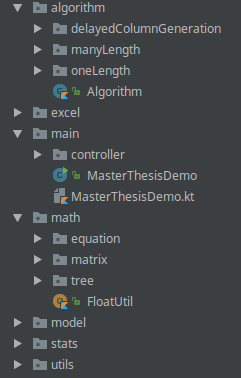
\includegraphics[scale=0.65]{../image/arch.png}
  \caption{Architektura aplikacji}
  \label{fig:arch}
\end{figure}

\begin{figure}[h]
  \center
  \includegraphics[scale=0.6]{../image/app_arch.png}
  \caption{Relacja między głównymi modułami aplikacji}
  \label{fig:app_arch}
\end{figure}

Architektura modułu odpowiedzialnego za implementację algorytmów posiada strukturę wzorca projektowego fasada. Klasy odpowiedzialne za konkretną implementację metody obliczenia rozkrojów rozszerzają klasę abstarkacyjną która definiuje wspólne funkcje oraz deklaruje metody które powinny zostać zdefiniowane w klasach potomnych. Główny moduł aplikacji wraz z modułem odpowiedzialnym za model danych tworzy implementację wzoraca Model-Widok-Kontroler (MVC). Klasa kontrolera zarządza widokiem stworzonym w języku FXML.

\hyperref[fig:java_arch]{Rynukek~\ref*{fig:app_arch}} opisuje korelację pomiędzy poszczególnymi modułami aplikacji wykorzystanymi do stworzenia programu z graficznym interfejsem użytkownika. Moduł Main odpowiedzialny jest za połączenie funkcjonalności aplikacji z GUI. Znajdują się w nim definicje widoku, wywołanie metod obliczających wynik z danych pobranych przez moduł excel oraz zapis rezultatu obliczeń. Moduł Model zawiera klasy odpowiedzialne za przechowywanie danych w aplikacji. Moduł Excel zawiera metody użyte do odczytu oraz zapisu danych w formacie CSV. Moduł Math zawiera operacje wykonywane na macierzach, jak również zawiera metodę do obliczania wartości nierówności metodą dwufazowej metody simplex, metodę podziału i ograniczeń do obliczenia wyniku całkowitego układu nierówności, metodę eliminacji Gaussa. W module tym znajduje się również klasa odpowiedzialna za tworzenie drzewa wykorzystanego przez metodę podziału i ograniczeń. Moduł Algorithm zawiera klasy odpowiedzialne za obliecznie schematu rozkroju z wykorzystaniem metod brutalnej siły oraz opóźnionej generacji kolumn.

Rysunki \ref{fig:empty_win} oraz \ref{fig:fill_win} przedstawiają okno aplikacji, odpowiednio przed wypełnieniem danymi oraz po zakończeniu obliczeń.

Program posiada możliwość wczytania danych z pliku CSV, a następnie zapisanie danych wyjściowych również do pliku CSV lub TXT. Kolejnymi zaimplementowanymi funkcjonalnościami są:
\begin{enumerate}
  \item wyświetlenie danych wejściowych oaz wyniku w oknie aplikacji
  \item wybór algorytmu rozkroju
  \item dodanie wielu długości podstawowych z różnym kosztem - domyślnie koszt jest równy długości.
  \item wyświetlenie długości podstawowych w oknie aplikacji
  \item dodanie szerkości cięcia dla metody brutalnej siły
\end{enumerate}

\begin{figure}[h]
  \center
  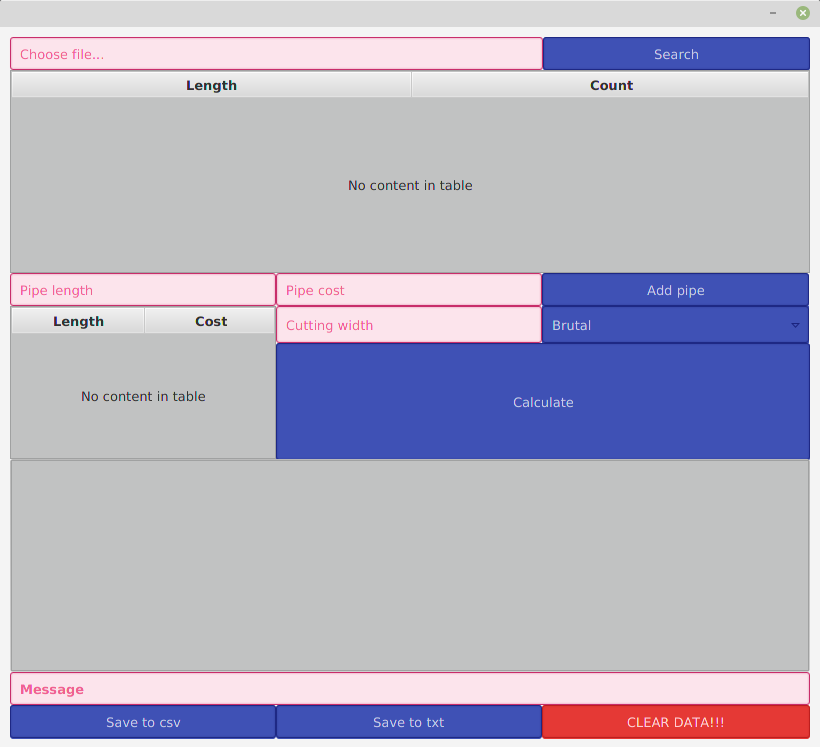
\includegraphics[scale=0.35]{../image/empty_win.png}
  \caption{Początkowe okno aplikacji}
  \label{fig:empty_win}
\end{figure}

\begin{figure}[H]
  \center
  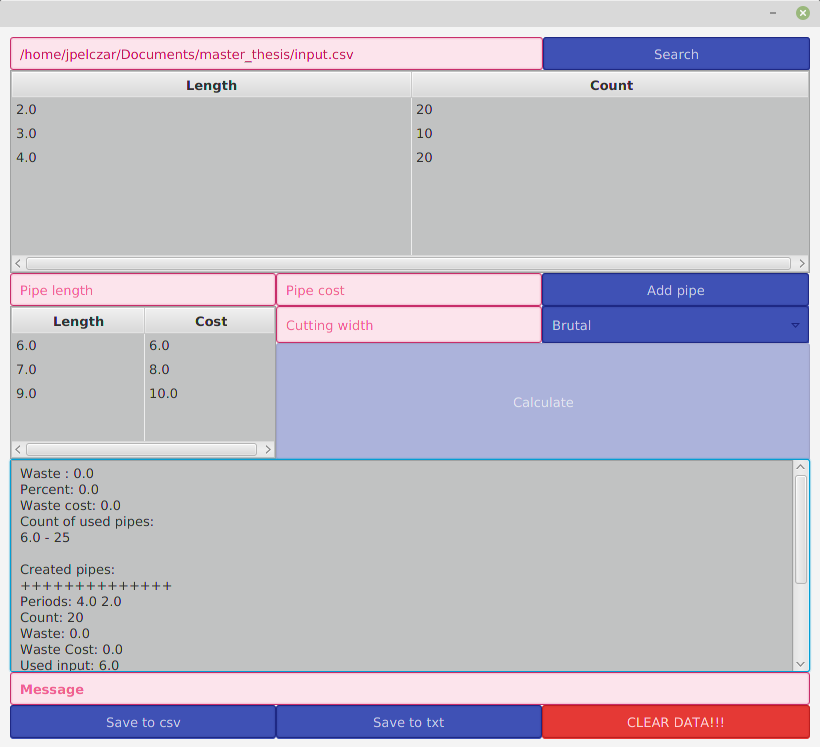
\includegraphics[scale=0.35]{../image/fill_win.png}
  \caption{Aplikacja po zakończonych obliczeniach}
  \label{fig:fill_win}
\end{figure}

\subsection{Java}
Język programowania Java jest językiem obiektowym z elementami programowania funkcyjnego wprowadzonymi od wersji 8. Aplikacje stworzone w tej technologii mogą być stosowane w różnych systemach operacyjnych, gdyż programy napisane w języku Java są kompilowane do plików class które umieszczane są w skompresowanej paczce jar. Pliki class następnie są przetwarzane przez maszynę wirtualną Javy (JVM - Java Virtual Machine) do postaci bytecode który jest wykonywany na urządzeniu. Istnieją implementacje JVM na większość używanych platform.

Tworzenie aplikacji w technologii Java jest możliwe poprzez użycie zestawu JDK (Java Development Kit). Uruchamianie tych aplikacji jest możliwe w środowisku JRE (Java Runtime Environment)  (\hyperref[fig:java_arch]{rys.~\ref*{fig:java_arch}}).

\begin{figure}[h]
  \center
  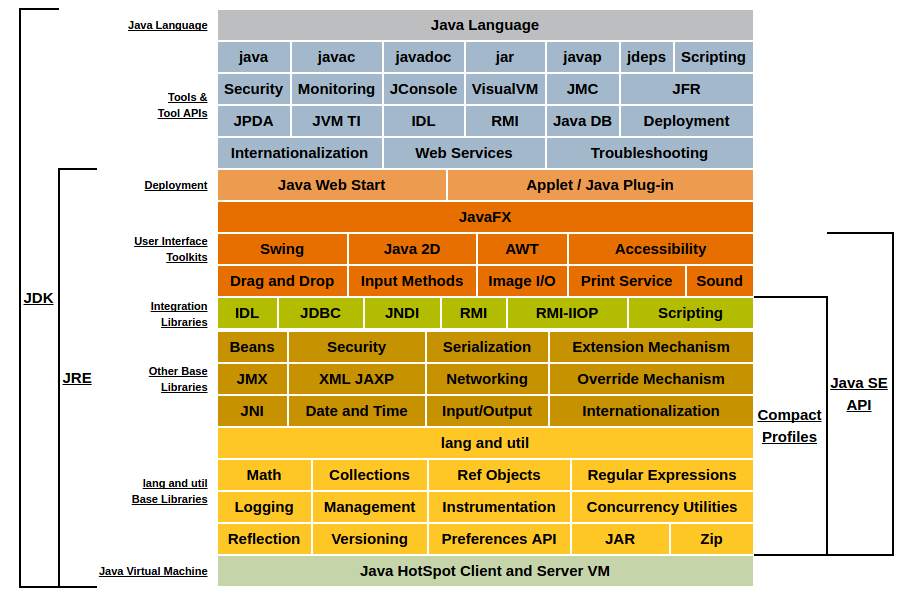
\includegraphics[scale=0.4]{../image/java_arch.png}
  \caption{Elementy składowe technologi Java \cite{OracleJavaArch}}
  \label{fig:java_arch}
\end{figure}

Podstawowym elementem technologii jest maszyna wirtualna. Jest to element technologii odpowiedzialny za niezależność programów od specyfikacji urządzenia oraz systemu operacyjnego. JVM jest abstarakcyjną maszyną obliczeniową. Podobnie jak rzeczywiste urządzenia posiada zestaw instrukcji pozwlających na sterowanie nią oraz wykonywanymi zadaniami. Maszyna wirtualna Javy nie zna języka Java, jedynie jego postać binarną zapisana w plikach class. Pliki te zawierają instrukcje dla JVM lub bytecode oraz inne wymagane informacje. Wiele języków programowania wykorzystuje tą cechę maszyny wirtualnej. Wymaganiem jest aby program był w postaci poprawnego pliku class, tak by mógł zostać wykonany na maszynie wirtualniej.

Technologia Java zawiera ponadto zestaw podstawowaych bibliotek pozwlających między innymi na budowanie plików JAR, refleksję czyli dostęp do metod oraz pól klasy bez zachowania zasad bezpieczeństwa, zdalne wywoływanie metod (RMI) oraz tworzenie graficznego interfejsu użytkownika Swing oraz AWT. Środowisko deweloperskie jest rozszerzone o narzędzia potrzebne do stworzenia programu, przykładowo: javac - kompilator przetwarzający pliki java do plików class, javadoc - narzędzie do tworzenia dokumentacji oraz język opisu interfejsów IDL służacy do komunikacji międzyprocesowej.
\subsection{JavaFX}
Zgodnie z (\hyperref[fig:java_arch]{rysunkiem~\ref*{fig:java_arch}}), JavaFX jest częścią standardowego API technologi Javy. Jest to zestaw graficznych i multimedialnych pakietów które mogą zostać wykorzystane do stowrzenia graficznego interfejsu użytkownika spójnego na przestrzeni wszystkich systemów operacyjnych \cite{JavaFxInfo}. Głównymi cechami tej technologii są:
\begin{enumerate}
  \item Zgodność z językiem programowania Java oraz możliwość współpracy z innymi językami JVM, takimi jak Scala, Kotlin lub JRuby.
  \item Język FXML który jest językiem znaczników bazujący na języku XML. Jest on wykorzystywany do opisu graficznego interfesju użytkownika, podobnie jak HTML.
  \item WebView jest to technologia wykorzystująca WebKitHTML która umożliwia zagnieżdzanie stron internetowych w aplikacjach JavaFX. JavaScript uruchominy w widoku strony internetowej może wywoływać metody dostępne w języku Java. Od wersji JavaFX 8 możliwa jest również obsługa HTML5.
  \item Istniejące aplikacje Swing mogą zostać zaktualizowane o możliwości JavaFX takie jak odtwarzanie treści multimedialnych oraz wyświetlanie stron internetowych.
  \item Wbudowana obsługa kaskadowych arkuszów stylów oraz komponentów intefejsu użytkownika umożliwia tworzenie spersonalizowanych aplikacji pod względem wyglądu interfejsu użytkownika.
  \item Obsługa grafiki 3D została dodana w wersji 8 JavaFX. Obiekty trójwymiarowe mogą być wyświetlane na odpowiednich z scenach z zastosowanym światłem. Klasa Camera odpowiedzialna jest za rendering widoku.
  \item Obsługa Canvas API umożliwia bezpośrednie rysowanie po obiekcie sceny która zawiera jeden element graficzny.
  \item Aplikacja zbudowana z Java oraz JavaFX jest umieszczona w paczce która może zostać uruchomiana na każdym urządzeniu które obsługuje wirtualną maszynę Javy.
  \item Ponadto JavaFX umożliwia obsługę drukowania, wielopunktowego dotyku oraz  wysokich rozdzielczości.
\end{enumerate}

  \begin{figure}[h]
    \center
    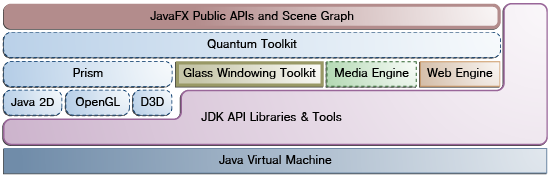
\includegraphics[scale=0.6]{../image/fx_arch.png}
    \caption{Architektura JavaFX}
    \label{fig:fx_arch}
  \end{figure}

\hyperref[fig:java_arch]{Rynukek~\ref*{fig:fx_arch}} opisuje architekturę technologi JavaFX. Zawiera ona zestaw deweloperski Java oraz maszynę wirtualną. Został również wyszczególniony silnik graficzny Prism odpowiedzialny za wyświetlanie widoków. Silnik ten może być wspomagany sprzętowo poprzez procesor graficzny. Na tym samym poziomie wraz z Prism znajduje się Glass Windowing Toolkik odpowiedzialny za współpracę z oknami systemowymi, zarządzaniu nimi oraz komunikację z systemowymi procesami odpowiedzialnymi za manipulację widokami. Prism, Glass Windowing Toolkit, silnik mutiledialny oraz internetowy współpracują ze sobą wykorzystując Quantum Toolkit który odpowiada za komunikację warstw powyżej z odpowiednimi elementami zarządzającymi grafiką.

\subsection{Kotlin}
Kotlin jest obiektowym językiem programowania który jest interpretowany do bytecode wywoływanego na maszynie wirtualnej Javy. Kotlin w porównaniu z Javą wnosi usprawnienia do programownaia proceduralnego. Kotlin jest zgodny z językiem Java, odnosi to skutek w możliwości łączenia obu języków programowania. Jest to technologia podobna do języka Scala jednak czas kompilacji został skrócony. Jest to język silnie rozwijający się w środowisku programistycznym Android. Dopiero najnowsza wersja narzędzi deweloperskich Android pozwala na wykorzystywanie niektórych elementów Javy 8. Kotlin zmniejsza liczbę nadmiarowego kodu potrzebnego do napisania przez programistę. Głównymi celami stworzenia technologii Kotlin były: pełna kompatybilność z językiem Java, zwiększenia bezpieczeństwa względem Javy (null safe), bardziej elastyczny oraz nieskomplikowany kod. Jedną z najciekawszych funkcjonalności języka Kotlin jest tworzenie metod rozszerzających daną klasę. Przykładowo może zostać zdefiniowana metoda $isNotEmpty()$ dla klasy $String$:
\lstset{language=Java}
\begin{lstlisting}[frame=single]
  fun String.isNotEmpty() = !this.isEmpty()
\end{lstlisting}
Metoda ta będzię dostępna dla każdego obiektu typu $String$ w programie.

\section{Zakończenie}
Problem optymalnego rozkroju rur jest szczegółowym przypadkiem problemu pleckaowego. Szczególne rozwiązania tego problemu mogą zostać osiągnięte na wiele sposobów. Porównanie dwóch algorytmów obliczania optymalnego rozkroju rur - brutalnej siły oraz opóźnionej generacji kolumn wskazuje na dwa typy metod. Obejmują one metody służące do prototypowania oraz do dokładnego obliczania wartości rozkroju. Metoda "Brutal Force" jest mniej skomplikowana oraz jest szybsza niż metoda "Delayed Column Generation", dlatego może zostać wykorzystana do szybkiego protypowania oraz przewidywania szacunkowych kosztów rozkroju. Druga metoda może zostać zastosowana do dokładnego obliczenia schematów rozkrojów. Schematy te mogą zawierać więcej elementów niż zostało zamówione lecz nadal posiadać mniejszy koszt niż metoda brutalnej siły.

Aplikacja udostępnia możliwość obliczania rozkrojów z własnych zamówień, zadanym algorytmem. Porównanie implementacji obu metod rozkroju potwierdziło, iż metoda brutalnej siły jest znacznie szybsza lecz wyniki są gorsze niż metody opóźnionej generacji kolumn. Implementacja programu wymaga wielu obliczeń macierzowych oraz wielu obliczeń wartości maksymalnej z układu nierówności. Są to operacje o bardzo dużym zapotrzebowaniu czasowym. Aplikacja może zostać rozszerzona o obsługę przypadku gdy w trakcie metody opóźnionej generacji wystepuje ujemna wartość kolumny liczebności danego rozkroju. Obecnie gdy taka sytuacja wystąpi zwracany jest ostatni znany poprawny rozkrój. W trakcie przeprowadzania eksperymentu, wyniki te zostały odrzucone ze względu na możliwość, iż sytuacja ta spowodowana jest losowymi danymi, które mogły mieć nieprawidłowy format wejściowy, lub ze względu iż przypadek ten został pominięty w implementacji. Kolejnym usprawnieniem aplikacji może zostać podzielenie obliczeń na wątki, tak aby praca został zrównoleglona oraz przyspieszona.

Rozszerzeniem algorytmu zastosowanego w metodzie opóźninej generacji kolumn może zostać metoda medianowa, zaproponowana przez Gilmorea oraz Gomorego \cite{GilmoreGomoryV2Article}. Metoda ta według przeprowadzonych eksperymentów może skrócić czas oraz obiżyć zapotrzebowanie na zasoby obliczeniowe nawet o 90\%.


\listoffigures
\bibliographystyle{abbrv}
\bibliography{praca_magisterska}

\end{document}
